\section{Formalization of Constant Time}
\label{sec:prelimnaries}

% State the technical details that are necessary to understand the paper. It is generally a collection of definitions, concepts and notations with potentially a few preliminary results. It can be, for example the mathematical framework in which the topic of your paper is expressed. In particular, fix the notation you will be using for your review.

Here we summarize the authors' formalization of constant-timedness for a simple, high-level, structured programming language. 
\figref{syntax} lists the language's syntax. 
The operational semantics for the language's primitives are standard and are listed in \figref{semantics} for reference.

\begin{figure}[h!]
  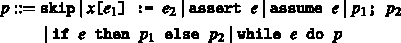
\includegraphics[width=\columnwidth]{figs/fig_5.pdf}
  \caption{Syntax of language used for formalization}
  \label{fig:syntax}
\end{figure}

\begin{figure}[h!]
  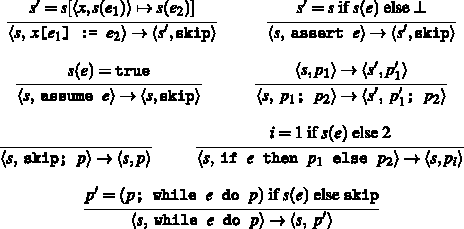
\includegraphics[width=\columnwidth]{figs/fig_6.pdf}
  \caption{Operational semantics of language in \figref{syntax}}
  \label{fig:semantics}
\end{figure}

\module{Modeling Program Execution:}
A state $s$ maps variables $x$ and indices $i \in $ to values $s(x,i)$ and we use $s(e)$ to denote the value of expression $e$ in state $s$. 
The distinguished error state $\bot$ represents a state from which no transition is enabled. A \emph{configuration} $c = \langle s,p \rangle$ is a state $s$ along with a program $p$ to be executed, and an \emph{execution} is a sequence $c_{1},c_{2},...c_{n}$ of configurations such that  $c_{i} \to c_{i+1}$ for $0<i<n$. The execution is \emph{safe} unless $c_{n} = \langle\bot,\mathunderscore\rangle$; it is \emph{complete} if $c_{n} = \langle\mathunderscore,skip\rangle$; and it is an \emph{execution of program p} if $c_{1} = \langle\mathunderscore,p\rangle$. A program $p$ is \emph{safe} if all of its executions are safe. 

Given a set of $X$ of program variables, two configurations $\langle s_1,
\_\rangle$ and $\langle s_2, \_ \rangle$ are \textit{X-equivalent} when
$\forall x \in X, i \in \mathbb{N}: s_1(x, i) = s_2(x, i)$. Executions 
$c_1 ... c_2$ and $c'_1 ... c'_n$ are initially \textit{X-equivalent} when 
$c_1$ and $c'_1$ are \textit{X-equivalent} and finally \textit{X-equivalent}
when $c_n$ and $c'_n$ are \textit{X-equivalent}.

\module{Modeling Leakages:}
A \emph{leakage model} $L$ maps program configurations $c$ to \emph{observations} $L(c)$, and extends to executions, mapping $c_{1},c_{2},...c_{n}$ to the \emph{observation} $L(c_{1},c_{2},...c_{n}) = L(c_{1})\cdot L(c_{2})\cdot\cdot\cdot L(c_{n})$. Two executions $\alpha$ and $\beta$ are \emph{indistinguishable} when $L(\alpha) = L(\beta)$.

\module{Definition of Constant-Time Security:} \emph{A program p with a set $X_{i}$ of inputs declared publicly observable and a set $X_{o}$ of  outputs declared publicly observable is constant-time secure when all of its initially $X_{i}$-equivalent and finally $X_{o}$-equivalent executions are executable.}

\module{Sources of leakage considered:} The authors consider three leakage models in this work---{(1)}~branch-based leakage,
{(2)}~memory access-based leakage, and
{(3)~leakage based on variable-latency instructions.

Branch-based leakages expose the valuations of branch conditions. For instance, here are the leakage models for branches in the example high-level language---
{(1)}~$\langle$ s, if e then $p_{1}$ else $p_{2}\rangle \mapsto s(e)$,
{(2)~$\langle$ s, while e do p$\rangle \mapsto s(e)$

Memory access-based leakages expose the addresses acccessed in load and store instructions. In the simple language of while programs this is equivalent to exposing the indexes to program variables read and written at each statement. 

Finally, the time required to execute an instruction may vary based on the provided operands on modern processors. For instance, integer division on x86 processors depends on the size of the two operands~\cite{intel-manual}). To account for such leakages, the authors add leakage models for all such instructions. Here, we only show the model for division - $\langle$ s, x = $e_{1}/e_{2}\rangle \mapsto sizeof(e_{1},e_{2})$

